\documentclass[10pt,a4paper,twocolumn]{article}
\usepackage[utf8]{inputenc}
\usepackage[portuguese]{babel}
\usepackage[T1]{fontenc}
\usepackage{apacite}
\usepackage{amsmath}
\usepackage{amsfonts}
\usepackage{amssymb}
\usepackage{tikz}
\usepackage{graphicx}
\usepackage{refstyle}
\usepackage{hyperref}
\usepackage{float}
\usepackage{natbib}
\usepackage{url}
\usepackage{listings}
\usepackage[export]{adjustbox}
\usepackage{xcolor}
\definecolor{ds}{rgb}{0.87,0.89,0.92}
\lstdefinestyle{mystyle}{
    backgroundcolor=\color{ds},   
    commentstyle=\color{red},
    keywordstyle=\color{magenta},
    numberstyle=\tiny\color{gray},
    stringstyle=\color{purple},
    basicstyle=\ttfamily\footnotesize,
    breakatwhitespace=false,       
    breaklines=true,                 
    captionpos=b,                    
    keepspaces=true,                 
    numbers=left,                    
    numbersep=5pt,                  
    showspaces=false,                
    showstringspaces=false,
    showtabs=false,                  
    tabsize=2
}
\lstset{style=mystyle}
\usepackage[left=2cm,right=2cm,top=2cm,bottom=2cm]{geometry}
\author{Sony Gonzaga de Melo Neto}
\title{Análise do Experimento das Oscilações Amortecidas\\
\large Universidade Federal de Campina Grande \\
  Disciplina: Instrumentação Científica \\
  Professor Adriano de A. Batista}
\hypersetup{colorlinks=true, linkcolor=blue}
\begin{document}
\maketitle
\section{INTRODUÇÃO}
Neste relatório será apresentada uma análise dos dados obtidos pelas oscilações de um Ressonador Mecânico. O objetivo é a determinação da frequência de oscilação do mesmo e seus fatores de decaimento e de qualidade, visto que seu comportamento é de um oscilador amortecido.\\
\par O Ressonador Mecânico é um dispositivo eletrônico capaz de gerar sinais elétricos oscilatórios. O mesmo, ao ser posto numa corrente elétrica, retorna-a oscilando com uma certa frequência. Podem ser construídos com um piezoelétrico que vibra ao receber a tensão, como também por um volume de ar confinado que ressoa enquanto está sobre a tensão, nesse caso, é chamado de Ressonador de Helmholtz. Suas aplicações, no geral, são em circuitos que requerem sinais periódicos.
\section{DESCRIÇÃO DO EXPERIMENTO}
O experimento foi realizado simplesmente aplicando uma tensão no Ressonador e o deixando oscilar por cerca de 10 segundos, enquanto sua amplitude diminuía. Os sinais retornados pelo equipamento foram registrados no computador, num arquivo .csv (Comma-separated values), e plotados num gráfico como a posição do elemento oscilatório no interior do Ressonador em função do tempo. O gráfico possui característica períodico de decaimento exponencial, podendo ser verificada sua semelhança com o oscilador subamortecido.
\section{O OSCILADOR AMORTECIDO}
O sistema de oscilação amortecida acontece quando há uma força dissipativa, proporcional à velocidade do objeto, que retira energia do sistema oscilatório a medida que o tempo passa. Seja pensado um sistema massa-mola, forças dissipativas possíveis seriam a resistência com o ar e o atrito de seus componentes mecânicos. 
\par A equação de movimento do oscilador amortecido para a posição é geralmente escrita como:
\begin{equation}
m\ddot{x}+\beta\dot{x}+kx=0.
\end{equation}
\par Dividindo todos os termos por $m$, sabendo que $\omega_0^2=\frac{k}{m}$, com $\omega_0$ a frequência ângular natural do sistema, e chamando $\gamma=\frac{\beta}{m}$ de fator de decaimento (pois está relacionado com a força dissipativa), a equação se torna:
\begin{equation}
\ddot{x}+\gamma\dot{x}+\omega_0^2x=0
\end{equation}
e sua solução é:
\begin{equation}
x(t)=Ae^{(-\gamma/2)t}\cos(\omega t+\phi),
\label{eq:x}
\end{equation}
com $A$ sendo o envelope de $x(t)$ e $\phi$ uma constante que depende das condições iniciais do sistema.
\par A frequência angular $\omega$ difere da frequência angular natural pela seguinte equação:
\begin{equation}
\omega=\sqrt{\omega_0^2-(\frac{\gamma}{2})^2}.
\label{eq:omega}
\end{equation}
\section{ANÁLISE DOS DADOS}
A série temporal dos dados foi plotada com um programa em Python, com a ajuda da biblioteca MatPlotLib. O script também executa a Transformada de Fourier e mostra seu gráfico para a análise das frequências que compõem a figura de oscilação. \par Abaixo, as referidas imagens para os dados brutos:
\begin{figure}[H]
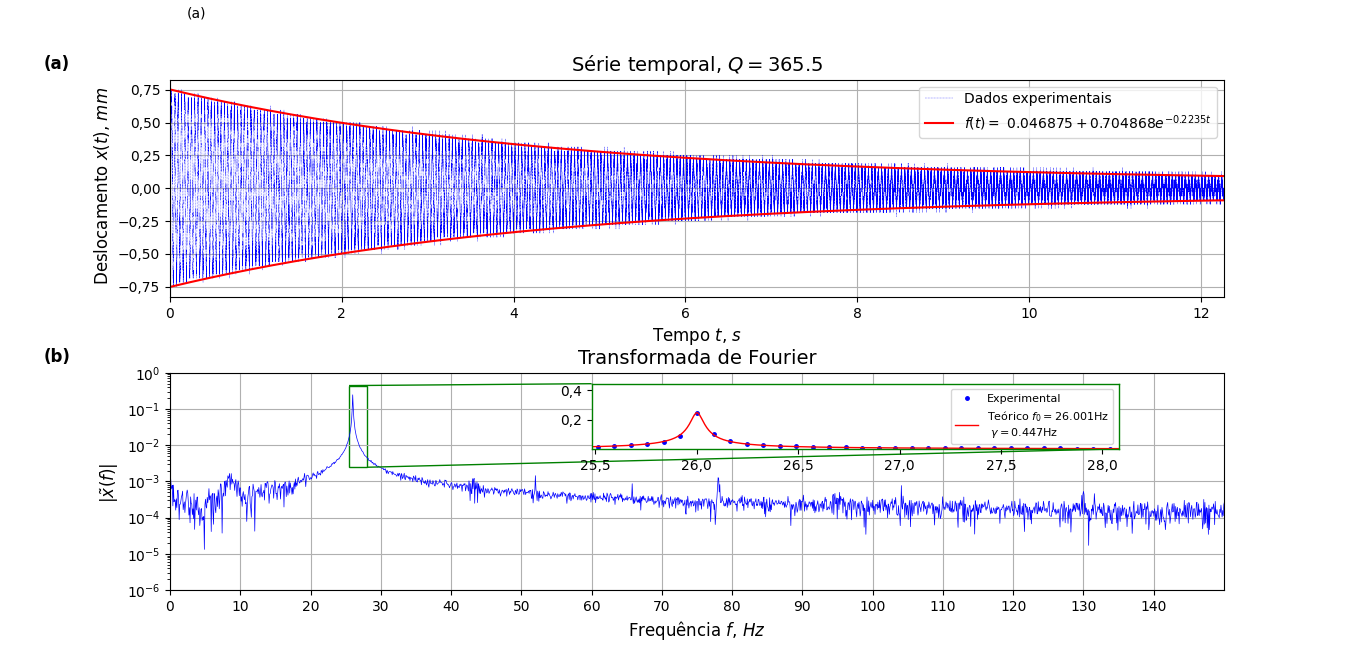
\includegraphics[width=0.5\textwidth, left]{NãoFiltrado}
\caption{Dados Brutos}
\label{fig:naofiltrado}
\end{figure}
\par O programa também retorna uma equação para o envelope exponencial $f(t)$ da oscilação amortecida, o fator de qualidade $Q$, a frequência natural de oscilação $f_0$ e o fator de decaimento $\gamma$, extraídos da Transformada de Fourier. Esses dados são obtidos ao se fazer uma aproximação pelos dois lados para $\gamma$:
\par Sabendo que a T.F., nesse caso, é equacionada como $f(\omega)=\frac{1}{\sqrt{(\omega^2-\omega_0^2)+\gamma^2\omega^2}}$, toma-se $\gamma_1$ e $\gamma_2$, tal que $\gamma_1<\gamma<\gamma_2$ e aproxima-se $\gamma_1$ de $\gamma_2$, calculando as raízes da equação $g(\gamma)=f(\gamma)-f(\gamma_1)+f(\gamma_2)$.
\par Entretanto, apesar da T.F. expressar os parâmetros procurados, a partir dos dados brutos, o envelope não reflete com precisão a real amplitude em função do tempo das oscilações. 
\par Para melhorá-la, faz-se o uso de um Filtro de Média Móvel, utilizando um programa escrito com a biblioteca Pandas, que atenua os ruídos e promove um série temporal mais limpa. O Filtro funciona seguindo a seguinte equação, para um certo sinal t e uma janela $n$:
\begin{equation}
y[t]=\frac{1}{n}\sum_{k=0}^{n-1}x[t-k].
\end{equation}
\par Para um $n$ muito pequeno, os ruídos pouco mudarão. Para $n$ muito grande, o gráfico perde sua característica oscilatória, portanto, cria-se um script com a biblioteca Scipy para encontrar o melhor $n$, determinando qual o menor valor de $\gamma$, pois o envelope é uma função do tipo $f(t)=C_1 + C_2e^{-(\gamma t)/2}$ e o fator de qualidade $Q=\frac{\omega_0}{\gamma}$ será o maior possível. 
\par Verifica-se que a função $\gamma(n)$ cresce para $n$ pequeno e para $n>512$, portanto, o script encontra o menor valor de maneira decrescente a partir de $n=512$, até achar um pico de mínimo em $n=414$, com $\gamma=0,446897314$. O gráfico da sequência temporal ao passar pelo Filtro de Média Móvel, fica, então:
\begin{figure}[H]
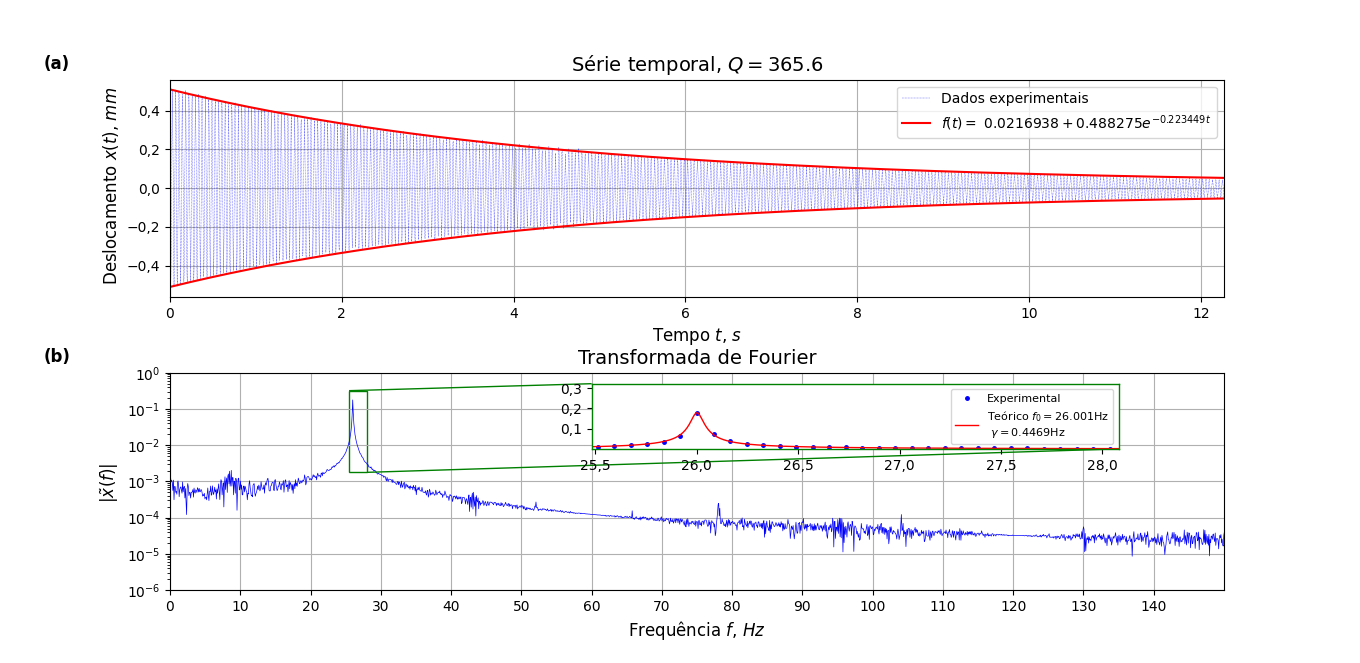
\includegraphics[width=0.5\textwidth, left]{Filtrado}
\caption{Dados filtrados com Filtro de Média Móvel}
\label{fig:filtrado}
\end{figure}
\par Por outro lado, como o Ressonador não desenvolve um movimento oscilatório ideal, este é aproximado e sua frequência encontrada pela T.F. não é satisfatória. Vê-se necessário truncar os dados para obter um intervalo da série temporal que melhor se aproxima do oscilador amortecido ideal. 
\par Para a obtenção de um bom valor aproximado da frequência natural, cria-se um script parecido com o anterior, mas que compare a frequência correspondentes a intervalos do final da série para passos decrescentes, ou seja, para truncamentos cada vez maiores. Obteve-se o melhor intervalo $9,32s<t<10,0s$ para uma frequência natural $f_0=26,4721 Hz$
\section{CONCLUSÃO}
O valor da frequência natural extraído da T.F. não ofereceu nenhuma variação considerável com a aplicação do Filtro. 
\par Substituindo os parâmetros obtidos da análise dos gráficos construídos com os dados da série temporal, $\gamma=0,446897314$ e $f_0=26,4721 Hz$ na equação \ref{eq:omega}, com $\omega=2\pi f$, a frequência das oscilações é $f=\frac{\omega}{2\pi}=26,4721 Hz$. A semelhança com $f_0$ se deve pelo fator de qualidade ser $Q=\frac{\omega_0}{\gamma}=372.19 >>1$.
\par A equação do gráfico de oscilações é, portanto, aplicando os parâmetros em \ref{eq:x} e o envelope $A=f(t)$,
\begin{equation}
x(t)=(0,0216938+0,488275e^{-0,223449t})cos(166,3291t+\phi).
\end{equation}
\par O gráfico abaixo mostra como a equação acima se comporta ao ser posta junto com os dados experimentais, tomando $\phi = 1.84 rad$:
\begin{figure}[H]
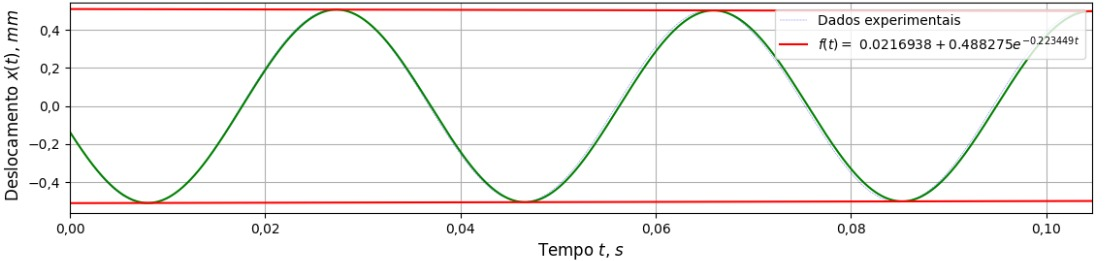
\includegraphics[width=0.5\textwidth, left]{Ajuste}
\caption{Ajuste da Série Temporal}
\label{fig:ajuste}
\end{figure}
\par Também é justo confirmar que, como $\omega_0 > \frac{\gamma}{2}$, o oscilador se encaixa no caso de subamortecido.

\newpage
\nocite{ressonador, nave, carlos2018, numpydoc, matplotdoc, pandasdoc, scipydoc}
\bibliographystyle{plainnat}
\bibliography{referencias}
\section{APÊNDICE}
\par Programas utilizados:
\lstinputlisting[language=Python, extendedchars=true,literate={á}{{\'a}}1 {ã}{{\~a}}1 {é}{{\'e}}1 {ó}{{\'o}}1 {Á}{{\'A}}1 {Ã}{{\~A}}1 {É}{{\'E}}1 {Ó}{{\'O}}1 {ç}{{\c c}}1 {í}{{\'i}}1 {ê}{{\^e}}1 {Ê}{{\^E}}1 {Ç}{{\c C}}1]{oscAmortecidasFTexpt.py}
\lstinputlisting[language=Python, extendedchars=true,literate={á}{{\'a}}1 {ã}{{\~a}}1 {é}{{\'e}}1 {ó}{{\'o}}1 {Á}{{\'A}}1 {Ã}{{\~A}}1 {É}{{\'E}}1 {Ó}{{\'O}}1 {ç}{{\c c}}1 {í}{{\'i}}1 {ê}{{\^e}}1 {Ê}{{\^E}}1 {Ç}{{\c C}}1]{plot_fft.py}
\end{document}